\title{Rokko Tutorial}

% 講習会名 (例: "CMSI柏ハンズオン")
\author{11th CMSI Young Researcher Technical Workshop}

% 講習会日時(4桁-2桁-2桁. 例: "2013-04-03")
\date{4th-6th, Feb 2015}

\newcommand{\RokkoRootDir}{/opt/hands-on/rokko}
\usepackage{graphicx}
\newcommand{\smallscr}[1]{\scalebox{0.4}{$#1$}}
\newcommand{\middlescr}[1]{\scalebox{0.60}{$#1$}}

\setbeamertemplate{note page}{\insertnote\par}

\setlength{\floatsep}{5pt plus 0pt minus 0pt}                                   
\setlength{\dblfloatsep}{5pt plus 0pt minus 0pt}  % 図表と図表の間のマージン(二段組みバージョン)
\setlength{\textfloatsep}{5pt plus 0pt minus 0pt}                               
\setlength{\dbltextfloatsep}{5pt plus 0pt minus 0pt} % 図表と本文の間のマージン 
\setlength{\intextsep}{5pt plus 0pt minus 0pt}                                  
\setlength{\abovecaptionskip}{5pt plus 0pt minus 0pt}   % 図表の caption と図表本体の間のマージン
\setlength{\belowcaptionskip}{5pt plus 0pt minus 0pt}   % 図表の caption 下部のマージン

\errorcontextlines=5

\newtheorem{rei}{Example}
\renewcommand{\therei}{}

\AtBeginSection[]{
    \begin{frame}
        \tableofcontents[currentsection]
    \end{frame}
}

\begin{document}

\lstset{language=c++,basicstyle=\ttfamily\tiny,showspaces=false,keepspaces=true,rulecolor=\color[cmyk]{0, 0.29,0.84,0}}

\begin{frame}
  \titlepage
  \noindent {\footnotesize PDF file: \url{http://sf.net/projects/rokko-tutorial/files/long-tutorial-en.pdf}} \\
  \noindent {\footnotesize LaTeX source: \url{http://github.com/cmsi/rokko-tutorial/wakate}}
\end{frame}

%% \section*{Outline}
%% \begin{frame}
%%   \tableofcontents
%% \end{frame}


\section{Eigenvalue Algorithms / Solvers, Linear Algebra Libraries}


\begin{frame}
  \frametitle{Matrix diagonalization}
  \begin{itemize}
    %\setlength{\itemsep}{1em}
  \item Matrix type
    \begin{itemize}
    \item real symmetric matrix, real unsymmetric matrix, complex Hermitian matrix, complex non-Hermitian matrix
    \end{itemize}
  \item Type of matrix storage
    \begin{itemize}
      \item dense matrix, CRS (Compressed Row Storage) format, MatFree\\
            (corresponding to ``small'', ``middle'', ``large'' in TITPACK2 resp.)
    \end{itemize}
  \item Eigenvalues to be computed
    \begin{itemize}
      \item all or the greatest (least) ones in absolute value, ones in some region
    \end{itemize}
  \item Eigenvectors
    \begin{itemize}
      \item wanted/unwanted
    \end{itemize}
  \end{itemize}
\end{frame}

\begin{frame}
  \frametitle{Definitions of Terms}
  \begin{itemize}
    %\setlength{\itemsep}{1em}
  \item Eigenvalue algorithm
  \item Eigensolver (solver for eigenvalue problem)
    \begin{itemize}
      \item Implementation of eigenvalue algorithm
    \end{itemize}
  \item Eigensolver Library
    \begin{itemize}
      \item a library which consists of only eigensolvers
    \end{itemize}
  \item Linear Algebra Library
    \begin{itemize}
      \item collection of eigensolvers and other solvers
    \end{itemize}
  \item Exact diagonalization package
    \begin{itemize}
      \item Software to deal with eigenvalue problems of Hamiltonian matrix for the quantum lattice model
    \end{itemize}
  \end{itemize}
\end{frame}

\begin{frame}
  \frametitle{Eigenvalue algortihm (part)}
  \begin{itemize}
    %\setlength{\itemsep}{1em}
  \item Eigenvalue algorithms for tridiagonalized matrix
    \begin{itemize}
      \item bisection method, QR method, MR3 method, divide-conquer method+QR method
    \end{itemize}
  \item Direct diagonalization of dense matrix
    \begin{itemize}
      \item Jacobi method
    \end{itemize}
  \item Tridiagonalization of dense matrix
    \begin{itemize}
      \item Householder method
    \end{itemize}
  \item Direct diagonalization of sparse matrix
    \begin{itemize}
      \item power method, inverse power method, Rayleigh quotient iteration method, Jacobi-Davidson method, LOBPCG, Krylov-Schur method
    \end{itemize}
  \item Tridiagonalization of sparse matrix
    \begin{itemize}
      \item Lanczos method, Arnoldi method, Restart Lanczos, Thick-restart Lanczos method
    \end{itemize}
  \item Other methods
    \begin{itemize}
      \item Sakurai-Sugiura method
    \end{itemize}
  \end{itemize}
\end{frame}

\begin{frame}
  \frametitle{Eigenvalue Algothims}
  \begin{center}
    \includegraphics[height=0.45\textheight]{figure/AppliedNumericalLinearAlgebra.jpg} \ \
    \includegraphics[height=0.45\textheight]{figure/TheSymmetricEigenvalueProblem.jpg} \ \
    \includegraphics[height=0.45\textheight]{figure/SenkeikeisanNoSuri.jpg}  \ \
    \includegraphics[height=0.45\textheight]{figure/GyoretsuNoKoyuchi.jpg}
  \end{center}
\end{frame}

\begin{frame}
  \frametitle{Existing eigesolver libraries (for dense matrix)}
  \begin{itemize}
    %\setlength{\itemsep}{1em}
  \item \href{http://www.aics.riken.jp/labs/lpnctrt/EigenExa.html}{EigenExa}: dense solver
    \begin{itemize}
      \item Householder (tri-diagonalization, penta-diagonalization) + divide\&conquer + QR
    \end{itemize}
  \item \href{http://elpa.rzg.mpg.de}{ELPA}
    \begin{itemize}
      \item Householder + divide\&conquer method + QR
    \end{itemize}
  \end{itemize}
\end{frame}

%% \begin{frame}
%%   \frametitle{Existing eigesolver libraries (for sparse matrix)}
%%   \begin{itemize}
%%   \item \href{http://trilinos.org/packages/anasazi/}{Anasazi}: Mainly iteration solvers
%%     \begin{itemize}
%%       \item Krylov-Schur, Jacobi-Davidson, XXX-Davidson, LOBPCG, Implicit Riemannian Trust Region Method
%%     \end{itemize}
%%   \item \href{http://www.caam.rice.edu/software/ARPACK/}{ARPACK}
%%     \begin{itemize}
%%       \item Implicit Restarted Lanczos
%%     \end{itemize}
%%   \item \href{https://code.google.com/p/blopex/}{BLOPEX}
%%     \begin{itemize}
%%     \item Locally Optimal Block Preconditioned Conjugate Gradient Method (LOBPCG)
%%     \end{itemize}
%%   \item \href{http://www.grycap.upv.es/slepc/}{SLEPc}: Mainly iteration solvers, Need to select seq or MPI parallel in building time
%%     \begin{itemize}
%%       \item Krylov-Schur, Generalized Davidson, Jacobi-Davidson, Rayleigh Quotient Conjugate Gradient, Contour integral Sakurai-Sugiura, Power method, Subspace Itertation, Arnoldi (explicit restart), Lanczos (explicit restart) \\
%%     \end{itemize}
%%   \item \href{http://www.comp-phys.org/software/ietl/}{IETL}: iterative solvers included in ALPS
%%     \begin{itemize}
%%       \item Lanczos, etc.
%%     \end{itemize}
%%   \end{itemize}
%% \end{frame}

\begin{frame}
  \frametitle{Existing linear algebra libraries (for dense matrix)}
  \begin{itemize}
    %\setlength{\itemsep}{1em}
  \item Vendor's implementation of LAPACK and ScaLAPACK
    \begin{itemize}
    \item \href{https://developer.apple.com/library/mac/documentation/Performance/Conceptual/vecLib/Reference/reference.html}{Apple VecLib}: LAPACK
    \item Fujitsu SSLII: LAPACK, a part of ScaLAPACK(part), etc.
    \item \href{https://software.intel.com/en-us/mkl_11.1_ref}{Intel MKL}: LAPACK, ScaLAPACK
    \item
      \href{http://developer.amd.com/tools-and-sdks/cpu-development/amd-core-math-library-acml/}{ACML(AMD
        Core Math Library)}: LAPACK
    \item \href{http://www.openblas.net}{OpenBLAS}: BLAS + a part of LAPACK routines (sucessive implementation for GotoBLAS)

    \end{itemize}
  \item \href{http://www.netlib.org/lapack/}{Netlib LAPACK}: Reference implementation of LAPACK
    \begin{itemize}
      \item Householder+QR, Householder + divide\&conquer + QR, Householder+bisection method, Householder+MR3
    \end{itemize}
  \item \href{http://www.netlib.org/scalapack/}{Netlib ScaLAPACK}: Reference implmentation of ScaLAPACK
    \begin{itemize}
      \item Householder + QR, Householder + divide\&conquer + QR, Householder+bisection, Householder + MR3
    \end{itemize}
  \item \href{http://eigen.tuxfamily.org/}{Eigen3}: serial, thread parallelized for matrix-matrix product)
    \begin{itemize}
      \item Householder+QR
    \end{itemize}
%  \item \href{http://libelemental.org}{Elemental}:included eigensolvers ''MRRR'' works well, only for square processes.
%    \begin{itemize}
%      \item Householder+MR3
%    \end{itemize}
  \end{itemize}
\end{frame}

%% \begin{frame}
%%   \frametitle{Existing linear algebra libraries (for sparse matrix)}
%%   \begin{itemize}
%%     %\setlength{\itemsep}{1em}
%%   \item \href{http://trilinos.org}{Trilinos}: It includes eigensolvers Anasazi.
%%   \item Xabclib (\href{http://ppopenhpc.cc.u-tokyo.ac.jp/}{ppOpen AT})
%%   \end{itemize}
%% \end{frame}

\begin{frame}
  \frametitle{Recommnded order}
  \begin{itemize}
    %\setlength{\itemsep}{1em}
  \item For dense matrix (seq.)
    \begin{itemize}
      \item LAPACK (vendor impl.) $>$ Eigen3
    \end{itemize}
  \item For dense matrix (MPI)
    \begin{itemize}
      \item EigenExa $>$ ELPA $>$ ScaLAPACK (vendor impl.) %$>$ Elemental
    \end{itemize}
  %% \item For sparse matrix (seq. MPI)
  %%   \begin{itemize}
  %%     \item Anasazi $>$ SLEPc
  %%   \end{itemize}
  \end{itemize}
\end{frame}

\begin{frame}
  \frametitle{Latest eigensolvers}
  \begin{itemize}
    \setlength{\itemsep}{1em}
  \item There are several hybrid-parallized(MPI+OpenMP) eigensolvers.
  \item It's almost impossible for users to implement parallel eigensolvers by themselves.
  \item Utilize open source hybrid-parallelized eigensolvers.
  \end{itemize}
\end{frame}

\begin{frame}
  \frametitle{Existing Exact diagonalization package}
  \begin{itemize}
    \setlength{\itemsep}{1em}
  \item Popular packages
    \begin{itemize}
    \item \href{http://alps.comp-phys.org/mediawiki/index.php/Main_Page}{ALPS} (\href{http://alps.comp-phys.org/static/software/applications/diag/fulldiag/doc/}{fulldiag} / \href{http://alps.comp-phys.org/mediawiki/index.php/Documentation:sparsediag}{sparsediag}): It uses LAPACK, IETL.
    \item \href{http://quattro.phys.sci.kobe-u.ac.jp/Kobe_Pack/Kobe_Pack.html}{KOBEPACK}: It includes their own eigensolvers
    \item \href{http://www-e.uni-magdeburg.de/jschulen/spin/}{SPINPACK}: It use LAPACK
    \item \href{http://www.noc.titech.ac.jp/~phys0016_nishimori/titpack2_new/index-e.html}{TITPACK2}: It includes their own eigensolvers
    \end{itemize}
  \item Serial or thread parallelized. No MPI parallelized.
  \item It makes calculations for a large number of sites difficult.
  \end{itemize}
\end{frame}

\section{Overview and Structure of Rokko}

\begin{frame}
  \frametitle{Problems in using existing eigensolvers}
  \begin{itemize}
    \setlength{\itemsep}{1em}
  \item Different designs (interface, block size, padding...) for different eigensolvers
  \item Documentation is insufficient.
  \item Different compiling / link options depending on architectures
  \item Linking problems between languages C++ / C / Fortran
  \item Complicated dependency among lower level libraries
  \item Users want rough estimate for performace of eigensolvers before trying it.
  \end{itemize}
\end{frame}

\begin{frame}
  \frametitle{Dependency of parallel dense solvers}
  \begin{center}
    \includegraphics[height=0.8\textheight]{figure/eigensolver_dependency.pdf}
  \end{center}
\end{frame}

\begin{frame}
  \frametitle{Delvelopers of Rokko}
  \begin{itemize}
    \setlength{\itemsep}{1em}
  \item Tatsuya Sakashita (ISSP, Tokyo Univ.) \ \href{mailto:t-sakashita@issp.u-tokyo.ac.jp}{t-sakashita@issp.u-tokyo.ac.jp}
  \item Ryo Igarashi (ISSP, Tokyo Univ.) \ \href{mailto:rigarash@issp.u-tokyo.ac.jp}{rigarash@issp.u-tokyo.ac.jp}
\item Yuichi Motoyama (ISSP, Tokyo Univ.) \ \href{mailto:y-motoyama@issp.u-tokyo.ac.jp}{y-motoyama@issp.u-tokyo.ac.jp}
  \item Tsuyoshi Okubo (ISSP, Tokyo Univ.) \ \href{mailto:t-okubo@issp.u-tokyo.ac.jp}{t-okubo@issp.u-tokyo.ac.jp}
  \item Synge Todo (Department of Physics / ISSP, Tokyo Univ.) \ \href{mailto:wistaria@phys.s.u-tokyo.ac.jp}{wistaria@phys.s.u-tokyo.ac.jp}
  \end{itemize}
\end{frame}

\begin{frame}
  \frametitle{Overview of Rokko}
  \begin{itemize}
    %\setlength{\itemsep}{1em}
  \item Language
    \begin{itemize}
      %\setlength{\itemsep}{1em}
    \item Core parts: C++
    \item Language binding: C, Fortran90
    \item Benchmarking script: Python
    \end{itemize}
  \item License
    \begin{itemize}
      %\setlength{\itemsep}{1em}
    \item Boost licene (almost freely available)
    \end{itemize}
  \item Source code
    \begin{itemize}
      %\setlength{\itemsep}{1em}
    \item Open to the public by GitHub\\
          \url{https://github.com/t-sakashita/rokko/}
    \end{itemize}
  \end{itemize}
\end{frame}


\begin{frame}
  \frametitle{Design Policy of Rokko}
  \begin{itemize}
    \setlength{\itemsep}{1em}
  \item Common vector and matrix class
  \item Absorb differences of individual solvers by wrappers
    \begin{itemize}
      %\setlength{\itemsep}{1em}
    \item As eigensolvers develop and change, we modify wrapping functions to keep Rokko's interface the same.
    \end{itemize}
  \item Without recompiling Rokko, you can select solver in runtime.
  \item Multiple solvers can be called at one program.
  \item Less overhead wrappers by using virutal functions and templates
  \item Available from C++, C, Fortran90
  \end{itemize}
\end{frame}

\begin{frame}
  \frametitle{Components of Rokko}
  \begin{itemize}
    %\setlength{\itemsep}{1em}
  \item Install scripts for eigenvalue solvers / linear algebra libraries
  \item Common fundamental classes (distributed matrix, process grid, etc.)
  \item Wrappers for eigensolvers (in C++)
  \item Factory for eigensolvers (in C++)
  \item C/Fortran wrapper
  \item Test/sample programs
  \item Benchmark scripts (future work)
  \end{itemize}
\end{frame}



\begin{frame}[c,fragile]
  \frametitle{Directory structure of Rokko}

\dirtree{%
 .1 \RokkoFilename{}.
 .2 \RokkoFilename{rokko}
 $\cdots$ Rokko body (header \& source files).
 .2 \RokkoFilename{sample}
 $\cdots$ Sample programs in C++.
 .3
 \href{https://github.com/t-sakashita/rokko/tree/develop/sample/dense}{dense}
 $\cdots$ for dense matrix ({seq.}\&MPI).
 .3 \href{https://github.com/t-sakashita/rokko/tree/develop/sample/sparse}{sparse} $\cdots$ for sparse matrix (MPI).
 .2 \href{https://github.com/t-sakashita/rokko/tree/develop/sample_c}{sample_c} $\cdots$ Sample programs in C.
 .3 \href{https://github.com/t-sakashita/rokko/tree/develop/sample_c/dense}{dense} $\cdots$ for dense matrix ({seq.}\&MPI).
 .3
 \href{https://github.com/t-sakashita/rokko/tree/develop/sample_c/sparse}{sparse}
 $\cdots$ spapse matrix (MPI).
 .2 \href{https://github.com/t-sakashita/rokko/tree/develop/sample_fortran}{sample_fortran}
 $\cdots$ Sample programs in Fortran.
 .3 \href{https://github.com/t-sakashita/rokko/tree/develop/sample_fortran/dense}{dense} $\cdots$ for dense matrix ({seq.}\&MPI).
 .3 \href{https://github.com/t-sakashita/rokko/tree/develop/sample_fortran/sparse}{sparse} $\cdots$ for sparse matrix (MPI).
% .2
% \href{https://github.com/t-sakashita/rokko/tree/develop/test}{test}
% $\cdots$ ctest用(インストール成否の確認).
% .2 3rd-party $\cdots$ 固有値ソルバ.
 .2 \href{https://github.com/t-sakashita/rokko/tree/develop/tutorial}{tutorial} $\cdots$ Tutorial.
 .3
 \href{https://github.com/t-sakashita/rokko/tree/develop/tutorial/titpack}{titpack}
 $\cdots$ Gradually rewriting TITPACK2 to use Rokko.
}

\end{frame}


\section{Parallel MPI dense eigensolvers}

\subsection{Basic concepts}

\begin{frame}
  \frametitle{2D process grid}
  \begin{itemize}
  \item Assigning MPI processes in 2-dimension
  \item Two types of majors: row-major / column-major
  \item Example: 4 processes (no. {\color{blue}0,1,2,3})
  \begin{figure}[htbp]
\begin{tabular}{cc}
\begin{minipage}{0.4\hsize}
\begin{center}
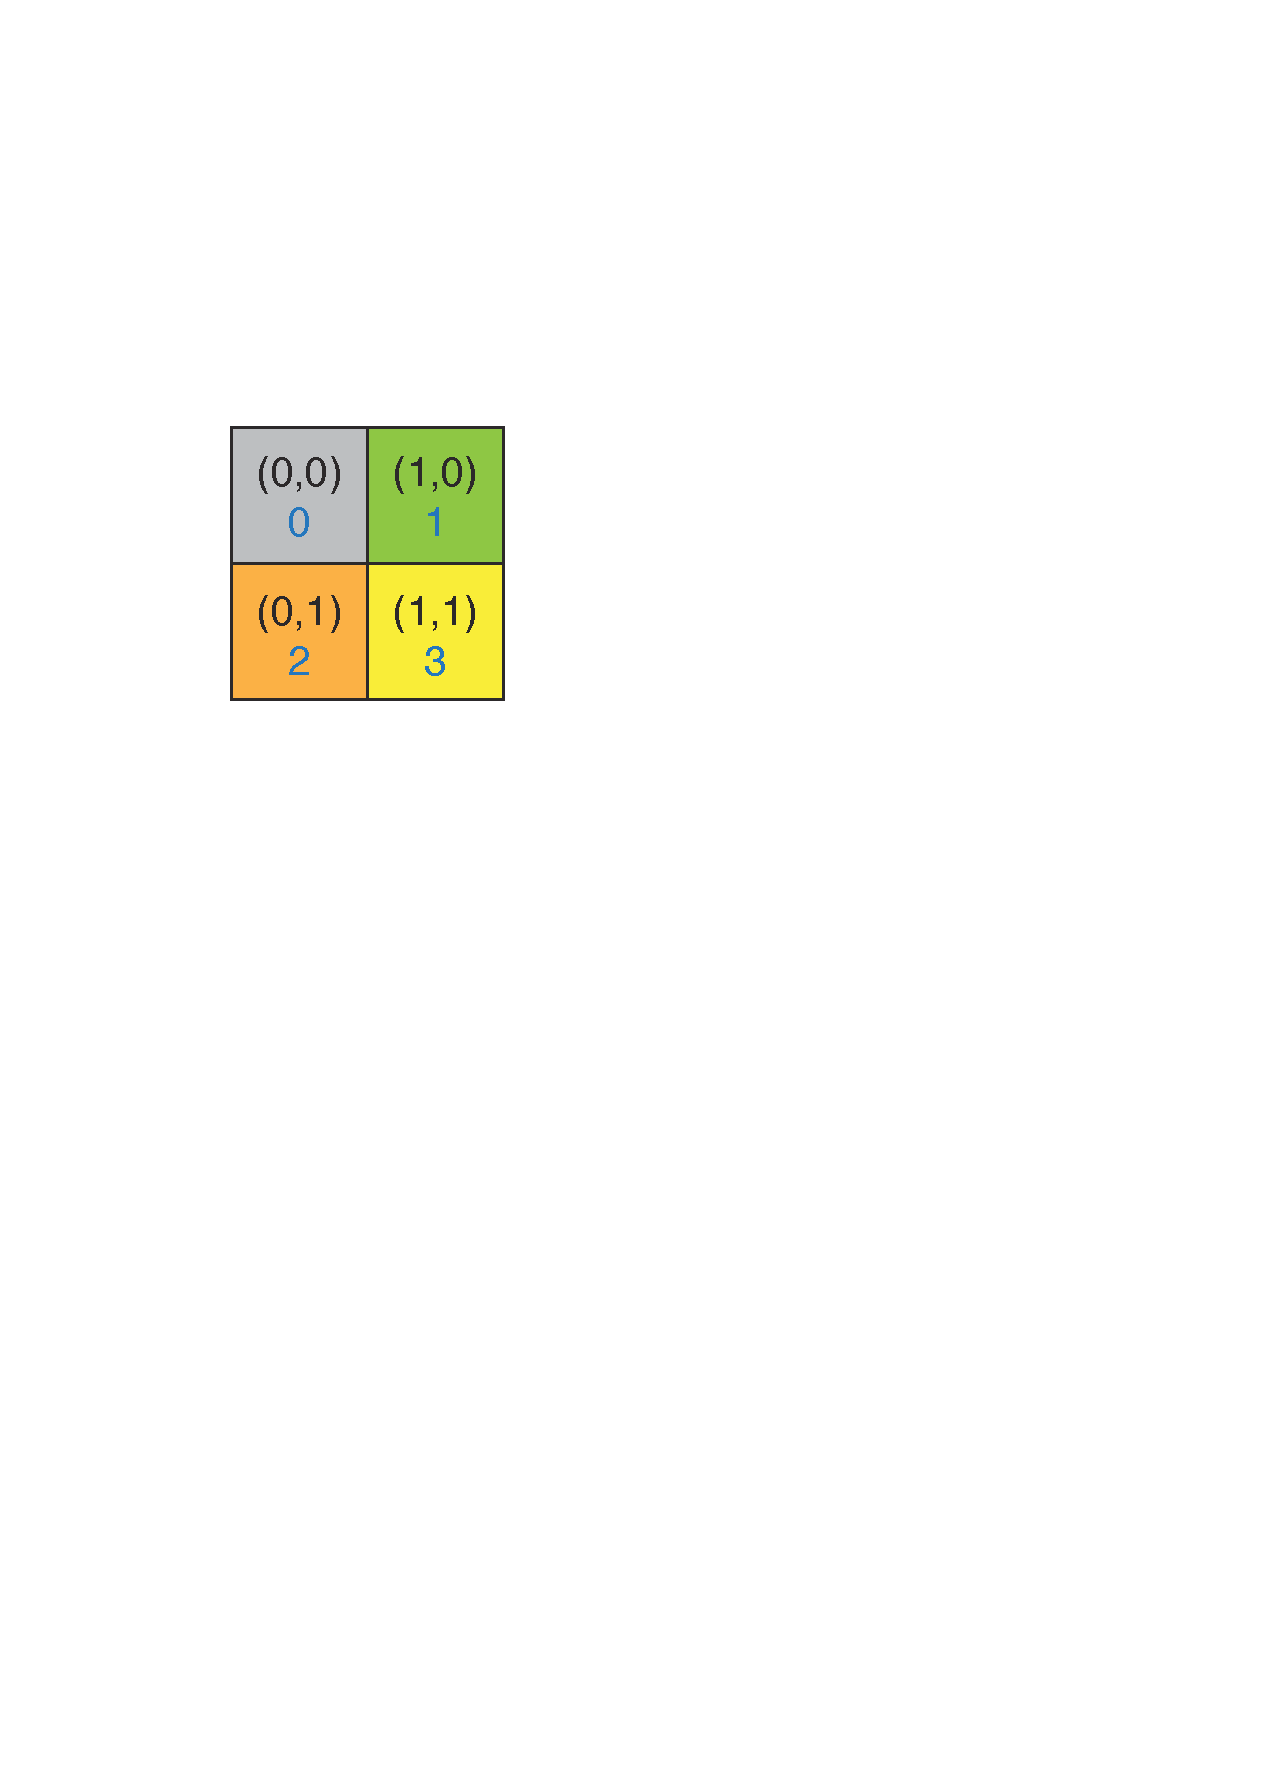
\includegraphics[height=0.25\textheight]{figure/grid-row-major.pdf}
\caption{row-major}
\label{fig:winter}
\end{center}
\end{minipage}
\begin{minipage}{0.4\hsize}
\begin{center}
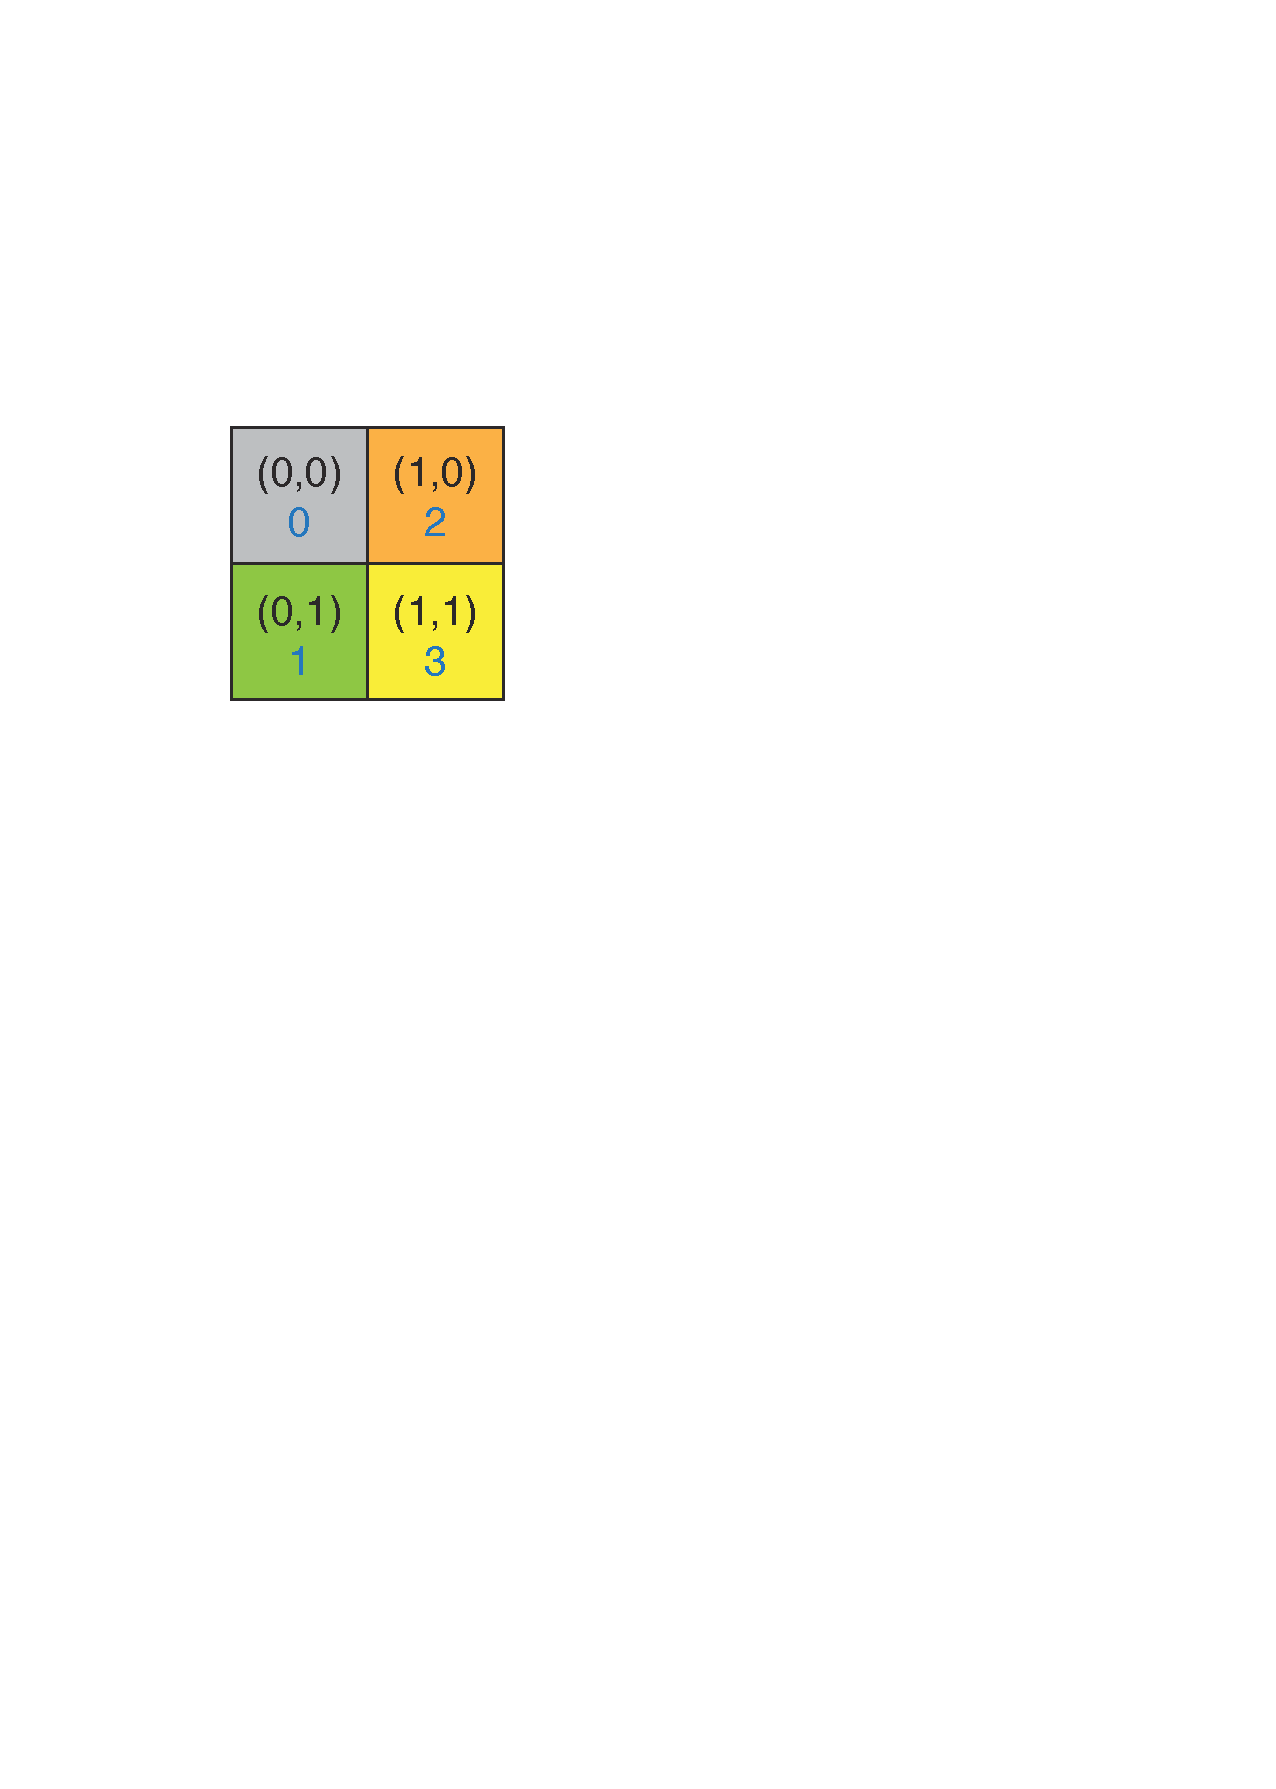
\includegraphics[height=0.25\textheight]{figure/grid-column-major.pdf}
\caption{column-major}
\label{fig:fall}
\end{center}
\end{minipage}
\end{tabular}
  \end{figure}
  \item All dense solvers support both grid majors.
  \end{itemize}
\end{frame}

\begin{frame}
  \frametitle{2-dimensional block cyclic matrix (distributed_matrix)}
  \begin{itemize}
    %\setlength{\itemsep}{1em}
  \item Parallel linear algebra libraries for dense matrices employ 2D process grid.
  \item Example (using the 2D process grid in the last page):
  \begin{figure}[htbp]
\begin{tabular}{cc}
\begin{minipage}{0.4\hsize}
\begin{center}
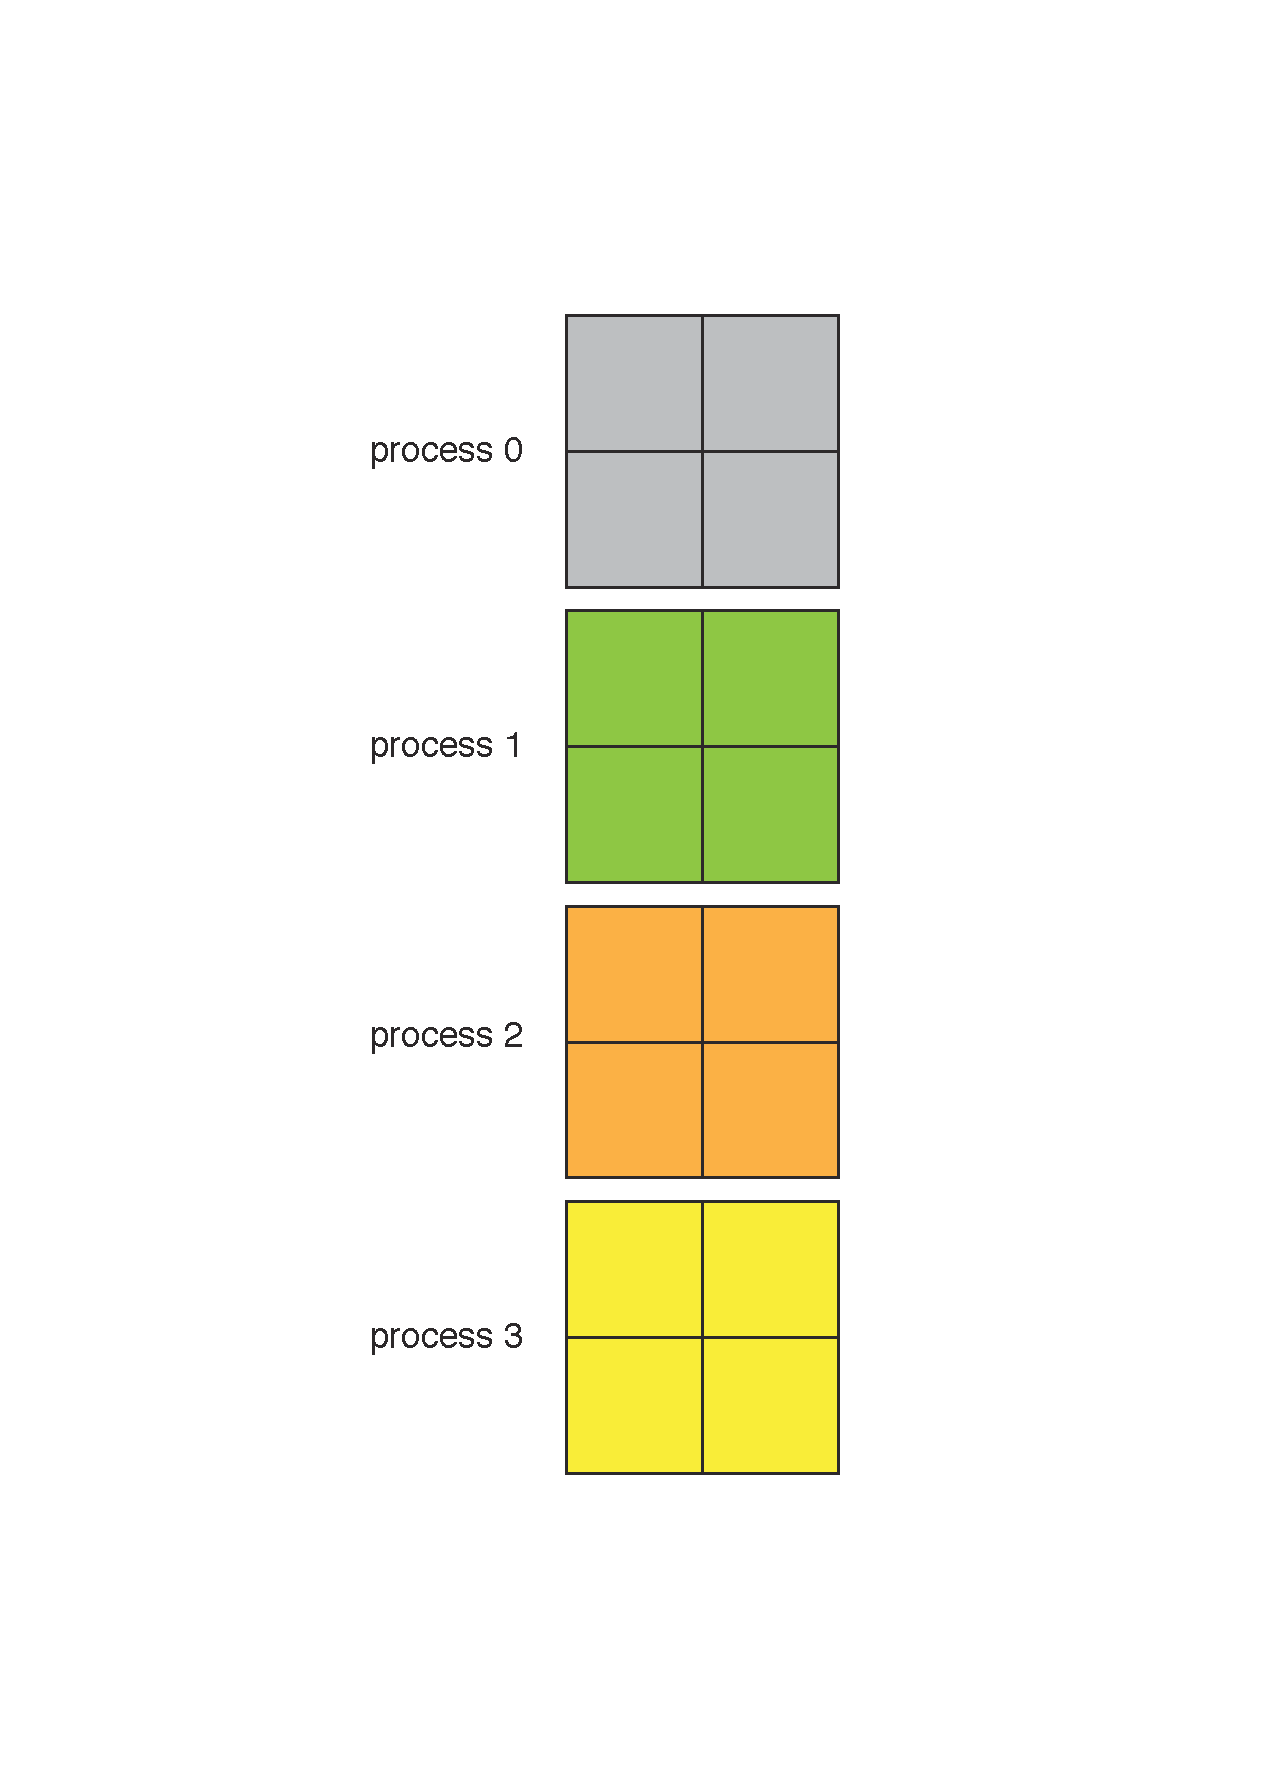
\includegraphics[height=0.45\textheight]{figure/local-view.pdf}
\caption{local view}
\label{fig:local-view}
\end{center}
\end{minipage}
\begin{minipage}{0.4\hsize}
\begin{center}
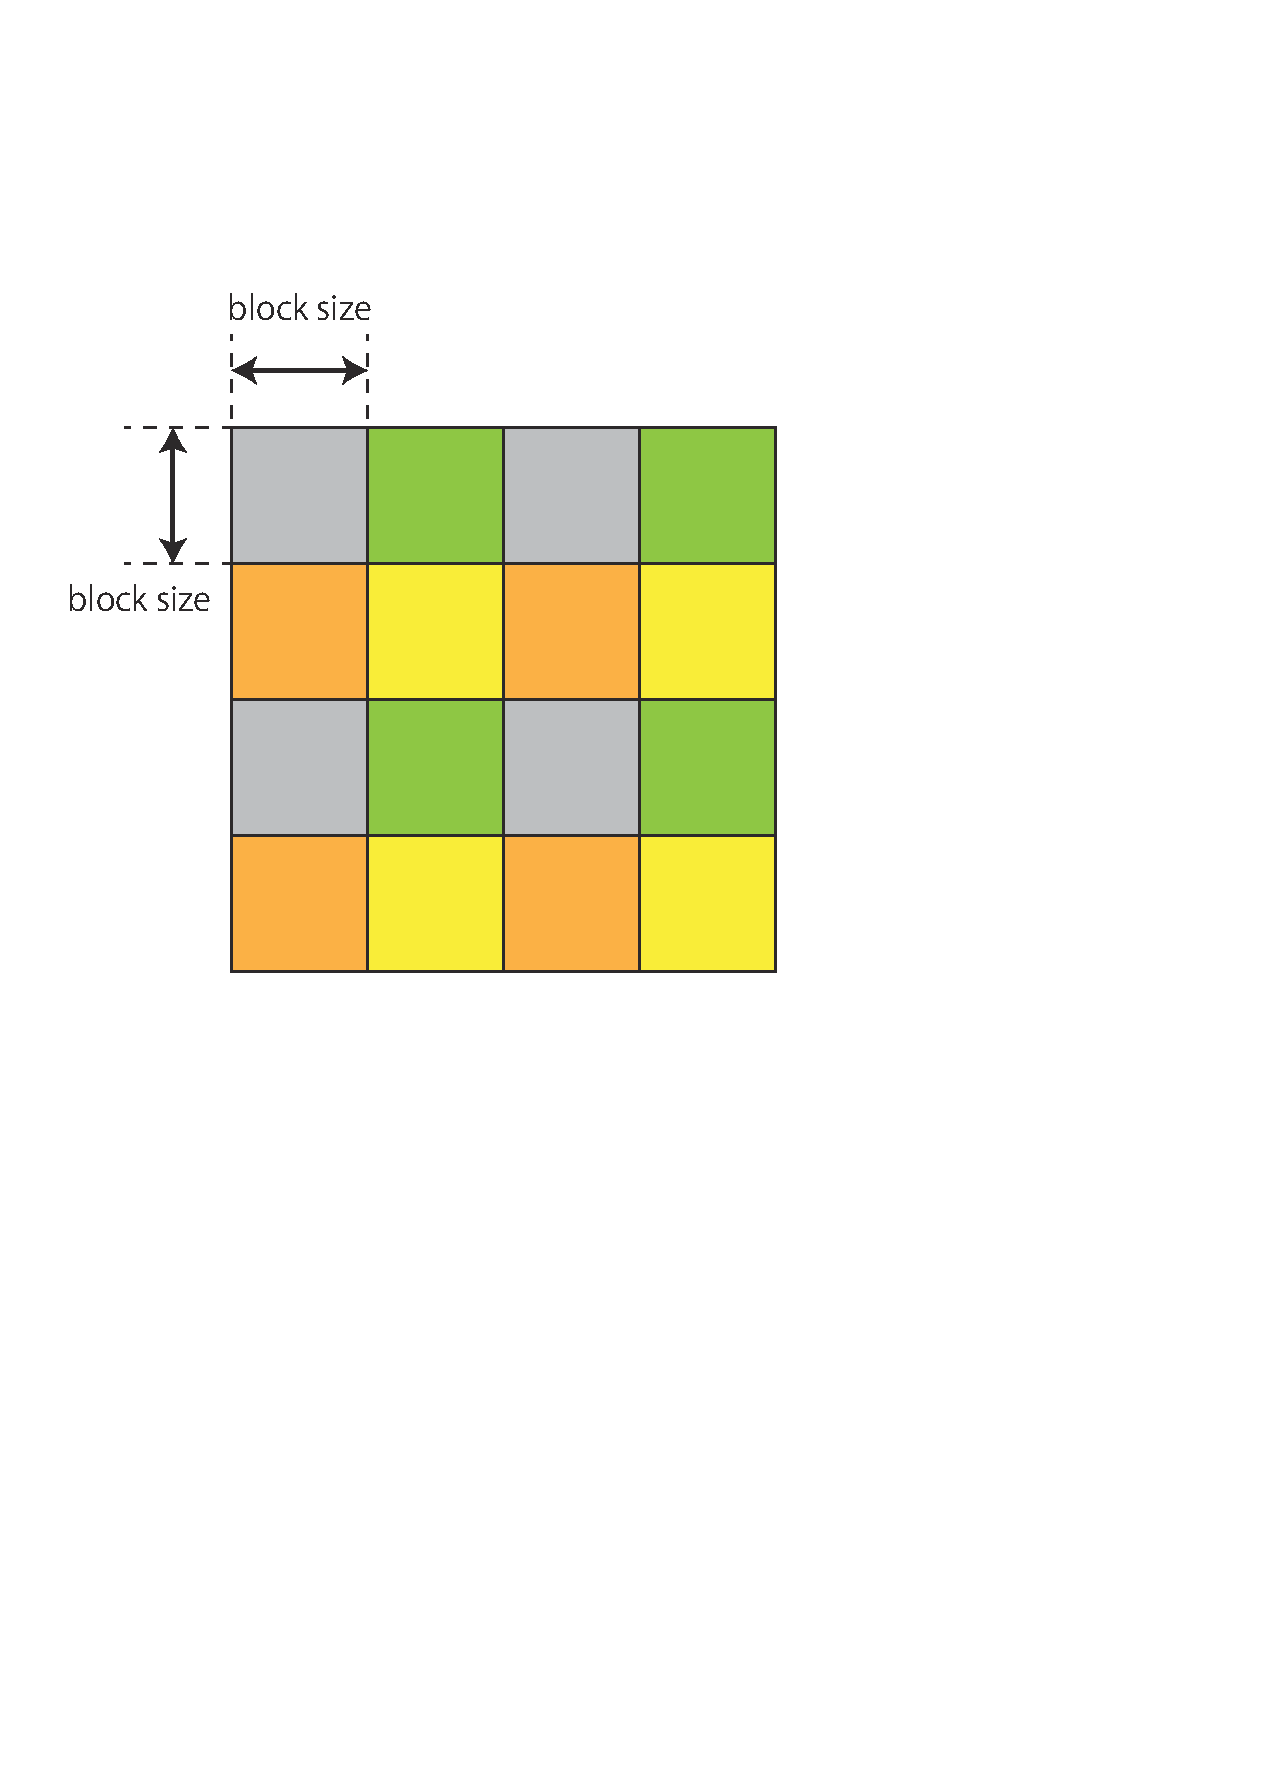
\includegraphics[height=0.45\textheight]{figure/global-view.pdf}
\caption{global view}
\label{fig:global-view}
\end{center}
\end{minipage}
\end{tabular}
  \end{figure}
  \item ScaLAPACK and ELPA support arbitrary block sizes.
  \item EigenExa support only $1 \times 1$.
  \end{itemize}
\end{frame}

%% \note{%
%% As far as I know, all eigensolvers for dense matrices empoly 2D block cyclic distributed matrix.
%% Not only eigensolvers, dense linear algebra libraries (such as linear equation solver, LU / QR decomposition) use block-cyclic distribution.

%% Block-cyclic distribution is decomposed way to squared tiles according to 2D process grid defined in the last slide. 
%% Each tile is assigned to one of processes in 2D process grid.
%% The size of squared tile is called block size.
%% The colors of tiles show assigned MPI processes.

%% As an example, I use 2D process grid appeared in the previous page.
%% Paving the whole matrix with the patterns of 2D process grids of given block size, you obtain block cyclic distribution.
%% It’s virtual global view.

%% Actual local storage is obtained by pulling out the same color tiles.
%% For example, the part of process 0 is obtained by pulling out the cyan-colored tiles.
%% Similarly, the part of process 1 is obtained by pulling out the green-colored tiles.

%% EigenExa support only 1x1 block size for computational efficiency.
%% }

\subsection{Specifications of Rokko interface}

\begin{frame}[c,fragile]
  \frametitle{LAPACK, ScaLAPACK, Rokko}
  \begin{center}
    \includegraphics[height=1.05\textheight]{lapack_scalapack_rokko.pdf}
  \end{center}
\end{frame}



\subsection{Run sample}


\begin{frame}[c,fragile]
  \frametitle{Test matrix: Frank matrix (definition)}
\begin{block}{Definition}
$[a_{ij}]_{i,j = {0, \dots, n-1}} = [ n - \max(i,j) ]$\\
\end{block}

\begin{block}{Example ($n=5$)}
$[a_{ij}]_{i,j = {0, \dots, 4}} =
\begin{bmatrix}
5 & 4 & 3 & 2 & 1 \\
4 & 4 & 3 & 2 & 1 \\
3 & 3 & 3 & 2 & 1 \\
2 & 2 & 2 & 2 & 1 \\
1 & 1 & 1 & 1 & 1 \\
\end{bmatrix}
$
\end{block}
\end{frame}

\begin{frame}[c,fragile]
  \frametitle{Test matrix: Frank matrix (properties)}
\begin{block}{Analytical eigenvalues}%
$\lambda_k = \dfrac{1}{2 \left( 1 - \cos{\tfrac{2 k + 1}{2 n + 1}\pi} \right)} \quad (k=0,\dots,n-1)$
\end{block}

\begin{block}{Remark}%
Frank matrix has an eigenvalue $1$\\
\quad $\Longleftrightarrow$ $\tfrac{2 k + 1}{2 n + 1} = \tfrac{1}{3}$\\
\quad $\Longleftrightarrow$ $n-1$ is a multiple of 3.
\end{block}
\end{frame}


\begin{frame}[c,fragile]
  \frametitle{Sample program for Frank matrix (dense matrix, MPI)}

  \begin{itemize}
%%     \item Preperation
%% \begin{lstlisting}[style=shstyle]
%% source /opt/MateriApps/env.sh
%% source /opt/MateriApps/rokko/rokkoenv.sh
%% \end{lstlisting}
    \item Source file: \href{https://github.com/t-sakashita/rokko/tree/master/sample/dense/frank_mpi.cpp}{frank_mpi.cpp}
    \item Command to run
\begin{lstlisting}[style=shstyle]
mpirun -np 4 ./frank_mpi eigen_exa_sx 10
\end{lstlisting}
    \begin{itemize}
    \item 1st argument: solver name ('eigen_exa_s', 'scalapack', 'scalapack_pdsyevd' is also available) \\
    \item 2nd argument: size of Frank matrix (The above example deals with $10\times 10$ size Frank matrix.)
    \end{itemize}
  \item Run by job script file /opt/wakate/rokko/script/frank_mpi.sh for psi.issp.u-tokyo.ac.jp
\begin{lstlisting}[style=shstyle]
cp -r /opt/wakate/rokko/script/ .
cd script
qsub frank_mpi.sh
\end{lstlisting}
  \end{itemize}
\end{frame}

\lstset{escapechar=\#}


\begin{frame}[c,fragile]
  \frametitle{Output result for Frank matrix (dense matrix, MPI)}
\setlength { \fboxrule } { 1.5pt }
\begin{lstlisting}[style=shstyle]
Eigenvalue decomposition of Frank matrix
num_procs = 4
num_threads per process = 12
solver = eigen_exa_sx
dimension = 10
largest eigenvalues: 44.766 5.0489 1.873 #\fcolorbox{red}{white}{1}# 0.6431 0.46523 0.36621 0.30798 0.27379 0.25568
residual of the largest eigenvalue/vector: |x A x - lambda| = 2.1316e-14
timer: enabled
timer: trace = disabled
timer: detailed report = disabled
timer:     1 solver::construct                                              0.000          1
timer:     2 solver::initialize                                             0.000          1
timer:     3 solver::finalize                                               0.000          1
timer:     4 diagonalize::initialize                                        0.217          1
timer:     5 diagonalize::diagonalize                                       0.961          1
timer:     6 diagonalize::finalize                                          0.000          1
timer:    10 main                                                           2.682          1
timer:    11 generate_matrix                                                0.051          1
timer:    12 output_results                                                 0.027          1
\end{lstlisting}
You can find an eigenvalue 1\\
$\longrightarrow$ The calculation result seems correct!
\end{frame}


\section{Diagonalization of Hamiltonian matrix for quantum spin system}

\begin{frame}[c,fragile]
  \frametitle{Quantum XYZ model}
\setlength{\fboxsep}{1pt}

\noindent
$\mathcal{H}
 := \sum\limits_{\middlescr{{\langle i,j \rangle}}} \left(
  J_x^{\smallscr{\langle i,j \rangle}} \, S^x_i \cdot S^x_j
+ J_y^{\smallscr{\langle i,j \rangle}} \, S^y_i \cdot S^y_j
+ J_z^{\smallscr{\langle i,j \rangle}} \, S^z_i \cdot S^z_j
\right)$

\vspace{1\baselineskip}

\noindent
$\mathcal{H}$ is written as an sum of local Hamiltonians:\\
\noindent
$\mathcal{H} =
\sum\limits_{\middlescr{\langle i,j \rangle}}  \mathcal{H}_{\smallscr{\langle i,j \rangle}}$ \\
$\text{where} \quad  H_{\smallscr{\langle i,j \rangle}} :=
\dfrac{1}{4}
\begin{bmatrix}
J_z & & & J_x-J_y \\
 & - J_z & J_x+J_y & \\
 & J_x+J_y & - J_z & \\
J_x-J_y & & & J_z
\end{bmatrix}$

\end{frame}


\begin{frame}[c,fragile]
  \frametitle{Sample program for Hamiltonian matrix of quantum XYZ model (dense matrix, MPI)}
%%   \item Heisenberg model (seq.) \RokkoFilename{sample/dense/heisenberg.cpp}
%% \begin{lstlisting}[style=shstyle]
%% ./sample/dense/heisenberg lapack
%% \end{lstlisting}
%%   \item Heisenberg model (MPI) \RokkoFilename{sample/dense/heisenberg_mpi.cpp}
%% \begin{lstlisting}[style=shstyle]
%% mpirun -np 4 ./sample/dense/heisenberg_mpi eigen_exa_sx
%% \end{lstlisting}
%%   \item XYZ model (seq.) \RokkoFilename{sample/dense/xyz.cpp}
%% \begin{lstlisting}[style=shstyle]
%% ./sample/dense/xyz_dense lapack $HOME/rokko-0.1/test/input_data/xyz_1hexagon.ip
%% \end{lstlisting}
  \begin{itemize}
%%   \item Preperation
%% \begin{lstlisting}[style=shstyle]
%% source /opt/MateriApps/env.sh
%% source /opt/MateriApps/rokko/rokkoenv.sh
%% \end{lstlisting}
    \item Source file: \href{https://github.com/t-sakashita/rokko/tree/master/sample/dense/xyz_mpi.cpp}{xyz_mpi.cpp}
    \item Command to run
\begin{lstlisting}[style=shstyle]
mpirun -np 4 ./xyz_mpi eigen_exa_sx ./xyz.dat
\end{lstlisting}
    \begin{itemize}
    \item 1st argument: solver name ('eigen_exa_s', 'scalapack', 'scalapack_pdsyevd' is also available) \\
    \item 2nd argument: input file (ref. next slide)
    \end{itemize}
  \item Run by job script file /opt/wakate/rokko/script/xyz_mpi.sh for psi.issp.u-tokyo.ac.jp
\begin{lstlisting}[style=shstyle]
cp -r /opt/wakate/rokko/script/ .
cd script
qsub xyz_mpi.sh
\end{lstlisting}
\end{itemize}
\end{frame}


\begin{frame}[c,fragile]
  \frametitle{Input file for Hamiltonian matrix of quantum XYZ model (dense matrix, MPI)}
xyz.dat
\begin{lstlisting}[style=shstyle]
8 8    #$\longleftarrow$number of sites, number of bonds#

0 1
1 2
2 3
3 4    #$\longleftarrow$ bonds $\langle i,j \rangle$ (pairs of site numbers)#
4 5
5 6
6 7
7 0

1.0 1.0 0.0
1.0 1.0 0.0
1.0 1.0 0.0
1.0 1.0 0.0
1.0 1.0 0.0    #$\longleftarrow
J_x^{\smallscr{\langle i,j \rangle}},\, 
J_y^{\smallscr{\langle i,j \rangle}},\,
J_z^{\smallscr{\langle i,j \rangle}}
$ for each bond ${\langle i,j \rangle}$#
1.0 1.0 0.0
1.0 1.0 0.0
1.0 1.0 0.0
\end{lstlisting}
\end{frame}

\begin{frame}[c,fragile]
  \frametitle{Output result for Hamiltonian matrix of quantum XYZ model (dense matrix, MPI)}
\begin{lstlisting}[style=shstyle]
Eigenvalue decomposition of XYZ model
num_procs = 4
num_threads per process = 12
solver = eigen_exa_sx
lattice file = ./xyz.dat
number of sites = 8
number of bonds = 8
dimension = 256
smallest eigenvalues: -2.6131 -2.4142 -2.4142 -1.8478 -1.8478 -1.8478 -1.8478 -1.8478 -1.8478 -1.7071
residual of the smallest eigenvalue/vector: |x A x - lambda| = 1.7764e-15
timer: enabled
timer: trace = disabled
timer: detailed report = disabled
timer:     1 solver::construct                                              0.000          1
timer:     2 solver::initialize                                             0.000          1
timer:     3 solver::finalize                                               0.000          1
timer:     4 diagonalize::initialize                                        0.204          1
timer:     5 diagonalize::diagonalize                                      24.244          1
timer:     6 diagonalize::finalize                                          0.000          1
timer:    10 main                                                          25.955          1
timer:    11 generate_matrix                                                0.045          1
timer:    12 output_results                                                 0.019          1
\end{lstlisting}
\end{frame}

\begin{frame}[c,fragile]
  \frametitle{Summary}
 \begin{itemize}
    \setlength{\itemsep}{1em}
  \item Review of existing eigensolvers
  \item Overview and Structure of Rokko
  \item Diagonalization of Hamiltonian matrix for quantum spin system
  \end{itemize}

  \begin{itemize}
  \item In this tutorial, we dealt with only MPI dense solvers
  \item Rokko has also interfaces for serial dense / MPI sparse solvers.
  \end{itemize}
\end{frame}


\end{document}

